
\newcommand{\figurewidth}[0]{1.8in}

\newcommand{\tablefig}[1]{
  \hspace*{-0.25in}
  \includegraphics[width=\figurewidth]{../graphs/graphs/#1}
}

\begin{figure}
\begin{center}
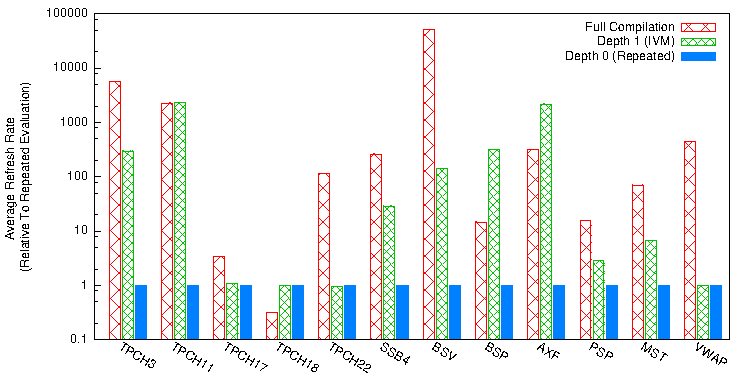
\includegraphics[width=3.4in]{../graphs/graphs/bakeoff.pdf}
\caption{Performance improvement achievable by our compiler.  Note the logscale on the y-axis. \comment{Detailed results for each query are presented below.}}
\label{fig:experiments:bakeoff}
\end{center}
\vspace*{-0.3in}
\end{figure}

We now analyze the performance of our compilation techniques and compare them with the results of Section 2.  Experiments are run on Redhat Enterprise Linux with 16 GB of RAM, and 2x4 core Intel Xeon E5620 2.4 GHz processors allocated to it.
\comment{Note that our compiler produces single-threaded code, while other engines were allowed to consume the full resources of the machine.} 
A query workload overview is presented in Section \ref{sec:sota}, and as SQL in Appendix~\ref{app:queries}.
\comment{Several stream traces were used to evaluate the queries.}
Queries were run over a replayed stream for 1 hour and then terminated. The results presented are computed based on the number of tuples processed within the 1 hour time limit.
\comment{Only those operations actually affecting the query results (e.g., VWAP's rate is computed based only on the number of operations on the BIDS table).}
Memory measurements are taken using google-perftools, and count memory allocated to the materialized views and not transient data.  

The financial queries VWAP, MST, AXF, BSP, PS, and BSV were run on a 2.63 million tuple trace of an order book update stream, representing of one day of stock market activity for MSFT.  These are updates to a BIDS and ASKS table with a schema of a timestamp, an order id, a broker id, a price, and a volume.  The stream consists of approximately 1.4 million operations on the BIDS table, and 1.14 million operations on the ASKS table.  

Queries from the TPC-H benchmark (including SSB4) were run on a scaling-factor 0.1 (100 MB) database generated by dbgen\cite{counciltpc}.  Additional scaling experiments were carried out on TPCH3 and TPCH11 at scaling factors 0.5, 1, 5, and 10, these results are presented in Section~\ref{sec:experiments:othermetrics}.  Insertions are drawn directly from the table files generated by dbgen and interleaved in random order.  Smaller datafiles finish earlier in the stream.  This provides insight into the performance characteristics of operations on different tables.

%SVL was run on a synthetically generated dataset, simulating 1000 racks of 20 servers each, emitting a total of 100,000 state updates.  The first 20,000 operations in the trace consist of an insertion for each server at 0 load.  For each state update, a random server deletes its previous state tuple and inserts a tuple declaring its new load -- a random real between 0 and 1.

To evaluate our compilation algorithm with a common performance baseline, we use a depth-limited instantiation of our compilation algorithm: Instead of recursively computing the entire materialization plan, the compiler stops after a fixed number of recursive steps.  Beyond this stage, queries are not materialized and instead computed directly from the base relations.   Compilation at depth-1 corresponds to traditional IVM techniques, and depth-0 corresponds to re-evaluating the query on every update.  Figure \ref{fig:experiments:bakeoff} provides end-to-end results of this comparison on our workload.

%As a consequence of the high join width of SSB4, the default materialization plan has an extremely high branching factor (12 at the top level).  Although most materialized views in the plan are duplicates, the compiler must still explore all children of unique nodes -- a prohibitively expensive process in our current compiler implementation.  For the purpose of these experiments, we omit deletions when compiling SSB4 (halving the branching factor).  As SSB4 is a query without nested aggregates, deletions are symmetric with insertions.  Hence the behavior of the two versions of the compiled query are identical for insert-only workloads.

\tinysection{Comparison with Existing Systems}
Figure \ref{fig:experiments:enginesVsDBT} compares our recursive compilation technique to the performance of the traditional databases and stream processors presented in Section~\ref{sec:sota} (and Figure~\ref{fig:queries}).  Recall that to reflect commensurate developer effort, CSPE and CDB were implemented using repeated evaluation (i.e., depth-0).  The performance disparity between our depth-0 implementation and the commercial systems is a result of the level of optimization these systems have undergone.  This bodes well for our technique, as it suggests that applying a similar level of optimization to our system can bring about a similar level of improvement not only for depth-0 but also for full compilation.

\subsection{Equijoins}

We first analyze the performance of our compiler on three equijoin queries without nested aggregates.  Our compiler recurs only once on TPCH11 (Figure \ref{fig:experiments:tpch3}b), and the result is nearly equivalent to IVM.  The fully compiled query materializes a projected and aggregated representation of SUPPLIER and PARTSUPP, but this provides only a minor improvement at this scale\footnote{Note however the results of Figure~\ref{fig:experiments:big}.}.  

Both TPCH3 and SSB4 (Figures \ref{fig:experiments:tpch3}a, and \ref{fig:experiments:ssb4}c) demonstrate a substantial performance increase over IVM.  The one-to-one and bounded fanout one-to-many relationships between elements of many of these queries are actually advantageous to the IVM implementation -- each insertion only triggers a limited number of reads.  In spite of this, incrementally maintaining the (aggregate) delta queries results in a net reduction in the amount of work required -- especially in a large query like SSB4.

Also note the memory usage of TPCH3.  Starting by the 40\%\ marker, all streams have been exhausted except for LINEITEM.  The final aggregate's group-by columns are drawn purely from the order table, so insertions into LINEITEM only update aggregate values for which entries have already been allocated by the corresponding ORDER.  Thus, memory usage plateaus for full compilation, while the IVM implementation must continue to store each row.

This is not always true.  For extremely large queries like SSB4 (a 7-way join), the number of intermediate materialized views created is quite large.  However, any individual update modifies only a small amount of that state -- the fully compiled query is substantially faster as long as the system has enough memory.  Memory usage is an important part of the cost/benefit tradeoff of full compilation, and we explore several other points in this space in Section~\ref{sec:experiments:othermetrics}.

\begin{figure}
\begin{center}
\resizebox{3.3in}{!}{
\begin{tabular}{|r|cccc|}\hline 
Query & Full Compilation & Depth 1 & CSPE & CDB\\ \hline 
{\bf TPCH3} & 27342.14 & 4.75 & 59.69 & 38.34\\ \hline 
{\bf TPCH11} & 44597.8 & 19.51 & XXX & XXX\\ \hline 
{\bf TPCH17} & 66.27 & 19.76 & 32.58 & 8.48\\ \hline 
{\bf TPCH18} & 1.95 & 6.13 & 21.13 & 38.07\\ \hline 
{\bf TPCH22} & 273.37 & 2.4 & 39.82 & 45.83\\ \hline 
{\bf SSB4} & 50.4 & 0.19 & 69.19 & 103.29\\ \hline 
{\bf BSV} & 110261.68 & 2.18 & XXX & XXX\\ \hline 
{\bf BSP} & 9.24 & 0.63 & 13.79 & 31.47\\ \hline 
{\bf AXF} & 54.15 & 0.17 & 12.28 & 31.1\\ \hline 
{\bf PSP} & 10.69 & 0.67 & 10.52 & 13.32\\ \hline 
{\bf MST} & 9.1 & 0.13 & 7.51 & 30.88\\ \hline 
{\bf VWAP} & 3259.47 & 7.4 & 9.31 & 12.89\\ \hline 
\end{tabular}
}
\caption{Comparison between the performance of our compiler and the two commercial query engines (in \# of refreshes per second) from Section \ref{sec:sota}.  These engines conceptually do the same amount of work as depth-0, but perform better as a result of commercial-grade optimization.  We expect a similar improvements to be possible for full compilation.}
\label{fig:experiments:enginesVsDBT}
\vspace*{-0.3in}
\end{center}
\end{figure}

\begin{figure*}
\begin{center}

\begin{minipage}{\textwidth}
\begin{center}
\hspace*{0.1in}
\begin{tabular}{cccc}
\tablefig{unified_tpch3.pdf} &
\tablefig{unified_tpch11.pdf} &
\tablefig{unified_ssb4.pdf} &
\tablefig{unified_tpch18.pdf} \\
(a) & (b) & (c) & (d)
\end{tabular} \vspace*{-0.2in}
\caption{TPCH3~(a), TPCH11~(b), SSB4~(c), and TPCH18 (d): (a) By the 40\%\ marker, all streams except LINEITEM have completed, and the remaining tuples consume no additional memory. (b) For simple two-way joins, full compilation is virtually identical to depth-1 and takes under 2 seconds, while depth-0 takes over an hour. (c) Full compilation is an order of magnitude faster than in IVC, although performance drops once the system begins running out of memory around the 27\%\ marker. (d) A badly chosen join ordering prevents full compilation from effectively exploiting foreign key dependencies in the TPC-H schema.}
\label{fig:experiments:tpch3}  
\label{fig:experiments:ssb4}
\label{fig:experiments:tpch11}
\label{fig:experiments:tpch18}
\end{center}
\end{minipage}

\vspace*{0.1in}

\begin{minipage}{\textwidth}
\hspace*{0.1in}
\begin{tabular}{cccc}
\tablefig{unified_brokervariance.pdf} & 
\tablefig{unified_vwap.pdf} &
\tablefig{unified_tpch17.pdf} &
\tablefig{unified_tpch22.pdf} \\
%\tablefig{unified_serverload.pdf} \\
(a) & (b) & (c) & (d)
\end{tabular} \vspace*{-0.2in}
\caption{BSV~(a), VWAP~(b), TPCH17~(c), and TPCH22~(d):  (a) The many-to-many relationship on the join term forces IVM to perform linear work on each insertion, which full compilation avoids. (b) IVM repeatedly re-evaluates the nested (parameterized) sub-query, while full compilation maintains a cache of sub-query results. (c) Due to the nested aggregate, IVC requires a nested loop, while full compilation requires only a single scan. (d) The small CUSTOMER stream completes at the 10\%\ marker, while the remaining ORDERS tuples require only linear time with full compilation. }
%(d) Materializing nested queries gains a polynomial degree of performance over IVM, but memory continues to grow. 
\label{fig:experiments:brokervariance}
\label{fig:experiments:tpch22}
\label{fig:experiments:vwap}
\label{fig:experiments:tpch17}
%\label{fig:experiments:serverload}
\end{minipage}

\vspace*{0.1in}

\begin{minipage}{\textwidth}
\hspace*{0.1in}
\begin{tabular}{cccc}
\tablefig{unified_pricespread.pdf} &
\tablefig{unified_missedtrades.pdf} &
\tablefig{unified_axfinder.pdf} &
\tablefig{unified_brokerspread.pdf} \\
(a) & (b) & (c) & (d)
\end{tabular} \vspace*{-0.2in}
\caption{PS~(a), MST~(b), AXF~(c) and BSP~(d):  (a,b) The performance and memory plateaus result from a portion of the trace from about 0.001\%\ to 0.01\%, where a single order is repeatedly placed and revoked. (c,d) Full compilation's aggressive materialization strategy results in the caches growing too large to be efficiently maintained.}
\label{fig:experiments:pricespread}
\label{fig:experiments:missedtrades}
\label{fig:experiments:axfinder}
\label{fig:experiments:brokerspread}
\end{minipage}

\end{center}
\end{figure*}


\subsection{Nested subqueries}

Figures \ref{fig:experiments:tpch17}b-d illustrate the performance of our compiler on several queries with nested aggregates.
The lookup over ORDERS in TPCH22 can be evaluated in constant time both using IVM and full compilation.  However each insertion into ORDERS incurs a nested aggregate on CUSTOMER, while full compilation materializes the aggregate result instead.

In IVM, insertions into CUSTOMER require two complete iterations over the customer table: once to compute the aggregate and once to figure out for which customers the state of the comparison changes.  The latter iteration cannot be eliminated by full compilation.  However, it need only iterate over the contents of the materialized view, which is already aggregated and projected down.

As with TPCH22, VWAP's uncorrelated aggregate can be evaluated efficiently if the query optimizer spots it -- the inequality-correlated aggregate is of more interest.  Because the domain of the correlating variable (price) is determined outside the nested aggregate, the nested subquery must be re-evaluated every time a new price is encountered.  However, the aggregate value can then be stored and incrementally maintained from that point on.  The domain of prices is bounded in practice, so after an initial ramp up process (that occurs while the size of the table is small) the fully compiled version can incrementally maintain the query output in (close to) constant time.

The performance of BSV (Figure \ref{fig:experiments:brokervariance}a) is similar to the prior two queries.  This is not surprising -- correlated aggregate subqueries are known to be equivalent to joins, and materializing a nested aggregate is tantamount to materializing the first delta.  Furthermore, unlike TPCH11 (Figure \ref{fig:experiments:tpch11}b), the join relationship is many-to-many, and the benefits of maintaining the join result as an aggregate grow over time.

As in the last several queries, incrementally maintaining the nested aggregate of TPCH17 makes insertions into PART constant-time rather than linear.  Even in the fully compiled version, insertions into the LINEITEM table must still iterate over the results of the join -- under full compilation this join has already been materialized.

\subsection{Other metrics}
\label{sec:experiments:othermetrics}

\tinysection{Limited Recursion}
\begin{figure}
\begin{center}
\resizebox{3.4in}{!}{
\begin{tabular}{|l|c|c|c|c|c|c|}\hline
{\bf Depth} & 1 & 2 & 3 & 4 & 5 & Full \\ \hline 
Avg Rate (refreshes/s) & 5.91 & 0.373 & 0.7 & 12.7 & 51.5 & 50.4 \\ \hline 
Avg Memory per Tuple & 98.5 B & 0.0 B & 0.0 B & 0.0 B & 0.0 B & 61.0 KB \\ \hline 
Lines of Code & 3174 & 12015 & 16517 & 13215 & 10998 & 10431 \\ \hline 
Number of Maps &        6 &       18 &       36 &       45 &       45 &       39 \\ \hline 
\end{tabular}
}
\caption{Statistics for different compilation depths on SSB4.  Depth-5 is equivalent to full compilation, but also maintains each of the 6 base relations.}
\label{fig:experiments:ssb4depth}
\end{center}
\vspace*{-0.2in}
\end{figure}
We now explore the space of limited recursive compilation beyond IVM.  Figure \ref{fig:experiments:ssb4depth} illustrates the effects of limiting compilation to depths between 0 and 5.  Recall that the maximum recursive depth is one less than the join width of the query.  Thus for SSB4 (which has a join width of 6), compilation to depth-5 is equivalent to full compilation, save that the base relations are materialized.

At depth-1, the compiled query materializes only the base relations and no intermediate tables.  It must still perform a 5-way join on every insertion, but  only once per update.  The 6 materialized views that it maintains are the 6 base relations from the query.  

At depth-2, the compiled query must now maintain 12 intermediate materialized views, several of which require a 4-way join to maintain.  The net cost of maintaining these additional views does not begin to pay off until depth-4 (where maintenance operations are reduced to at most 2-way joins).  By this point, decomposition has already resulted in the instantiation of all intermediate materializations relevant to the query, so extra and unnecessary work is being done.  

The effectiveness of this approach at depth-4 (in spite of the extra work) suggests that a more effective approach to reducing memory consumption might be to materialize not just the set of views closest to the root, but rather a subset of the possible materialized views.  However, the space of materialization strategies is exponential, and a cost based optimizer is future work.

\tinysection{Scaling}
Figure \ref{fig:experiments:big} analyzes how two queries: TPCH3 and TPCH11 scale to larger datasets.  Note that on TPCH3, the depth-1 implementation does not successfully complete the entire workload within the 1-hour time limit on any scaling factor greater than 0.1.  With full compilation, Query 3 consumes a large fraction of system memory on the 10 GB dataset, but performance remains constant throughout.  Query 11's performance also remains constant -- note the nearly 50\% improvement over IVM at higher scales, an effect of pushing aggregation into the materialized views.

\subsection{Memory, extraction, and future work}
\label{sec:experiments:future}

\begin{figure}
\begin{center}
\begin{tabular}{|l|c|c|c|}\hline 
\ & Infinite Depth & Depth 1 & Depth 0 \\\hline 
TPCH3 & 2509 & 2855 & 4198 \\\hline
TPCH11 & 531 & 596 & 616 \\\hline
TPCH17 & 928 & 1158 & 1478 \\\hline
TPCH18 & 3668 & 3538 & 4631 \\\hline
TPCH22 & 777 & 1135 & 754 \\\hline
SSB4 & 10995 & 8954 & 7904 \\\hline
BSV & 342 & 327 & 347 \\\hline
BSP & 45625 & 567 & 729 \\\hline
AXF & 2169 & 553 & 1394 \\\hline
PSP & 1442 & 1878 & 1890 \\\hline
MST & 5457 & 2870 & 2434 \\\hline
VWAP & 533 & 466 & 341 \\\hline
\end{tabular}
\caption{Lines of C++ generated for each query.}
\label{fig:experiments:loc}
\end{center}
\vspace*{-0.35in}
\end{figure}

It is important to understand not only where our compiler succeeds, but where its limitations lie.  We now consider several cases where the observed performance of our technique does not match our expectations.  As a consequence of our experimentation and analysis, we have identified three core challenges for future work in this area.

\tinysection{Join Ordering}
In spite of the simplicity of TPCH18 (Figure \ref{fig:experiments:tpch18}d), the query performs poorly -- even repeated evaluation is faster.  This is a consequence of our join ordering heuristic: The trigger that updates the query result must compute a join between the delta of the extracted nested subquery (aggregated over orderkey) and a materialized representation of CUSTOMER $\bowtie$ ORDER $\bowtie$ LINEITEM (aggregated over custkey and orderkey).  
Not knowing about the one-to-many relationship between custkey and orderkey, we iterate over the materialized join first and effectively iterate over all orders placed so far.
We ommitted a fully fledged join-ordering optimizer to focus our efforts on multilevel IVM. Adding join ordering during compilation is straightforward in functional optimization.
\comment{Join ordering is a well studied problem in the database community, and the solution to this problem is purely an engineering challenge.  A further outcome of the suboptimal join ordering is that the added (unnecessary) looping involves lookups that extend the domain of several intermediate materialized views, causing an explosion of memory use.}

\tinysection{Domain Maintenance}
Both PS and MST (Figures \ref{fig:experiments:pricespread}a, and \ref{fig:experiments:missedtrades}b respectively) do not perform as well as possible -- Apart from a stretch of updates (0.001\%\ to 0.01\%\ in the trace) in the stock market trace where the same order is repeatedly placed and revoked, query performance decreases polynomially over time.  This slowdown is due to overly aggressive caching.  We do not connect the domain of a materialized view's output variables with the domains of its base relations.  The effect of removing a row in the base relation is propagated to the multiplicity of the corresponding row(s) of the view.  However, the row itself is not garbage collected, and remains a part of iterations over the view.

\tinysection{Map Extraction}
The final case of performance issues is seen in both AXF (Figure \ref{fig:experiments:axfinder}c) and BSP (Figure \ref{fig:experiments:brokerspread}d).  Our aggressive extraction heuristic attempts to materialize the entire delta query, which for inequality joins includes an unbound variable.  The result of the delta query is a table with one entry for each broker.  However, the delta query also includes an unbound variable with a domain that is as large as either input table -- insertions into either table trigger maintenance work that is linear in the number of prior insertions onto the other table.  Worse still, the work saved by doing this is minimal -- the aggregate value must be computed from scratch on every insertion.

An improved, data-dependent extraction heuristic can identify such situations and compute the inequality join inline.  This is precisely what IVM is already doing -- hence the performance improvement.  Alternatively, the entire materialized delta could be incrementally maintained more efficiently using datastructures suited to computing aggregates over ranges (e.g., Range Trees\cite{rangequeries}).


\begin{figure}
\begin{center}
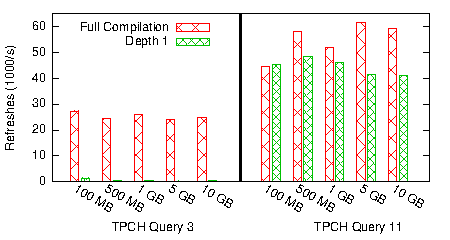
\includegraphics[width=3.4in]{../graphs/graphs/scaling.pdf} \\
\vspace{-3mm}
\caption{Performance scaling with respect to dataset size for TPCH 3 and 11 respectively.  For these queries, performance remains roughly constant as long as sufficient memory is available.}
%The three fastest-running TPC-H queries (3~(b), 11~(c), and 22~(d)) run on a 5GB dataset: (b) Quadratic effects from early parts of the workload become apparent in IVM at this scale, while full compilation remains linear. (c) Maintaining the base relations already projected and aggregated gives a slight edge to full compilation at this scale.  (d) Full compilation performance is reduced due to updates being linear in the size of CUSTOMER, but still performs better than depth 1.
\label{fig:experiments:big}
%\label{fig:experiments:big:tpch3}
%\label{fig:experiments:big:tpch11}
%\label{fig:experiments:big:tpch22}

\end{center}\vspace*{-0.3in}
\end{figure}



